% Generated by manuscript/build_manuscript.py.
\section{Problem Formulation and Empirical Motivation}
\label{sec:problem-formulation}


The preceding discussion shows that UVHF involves more than sharing parameters across prediction lengths. A unified forecaster should return coherent predictions for future steps shared by different horizon requests, while its decoder must determine how predictive information is shared across the future domain. We now formalize these two issues and examine them through controlled empirical analyses, which motivate the decoder design developed in Section 4.

\subsection{Unified varied-horizon forecasting and cross-horizon prefix consistency}


Consider two forecasting requests with horizons $H_i<H_j$ issued from the same observed history. Their first $H_i$ steps refer to identical future targets and should therefore receive identical predictions. We formalize this requirement below.

At forecast origin $o$, let

\[
\mathbf X_o
=
\left[\mathbf x_{o-L+1},\ldots,\mathbf x_o\right]
\in\mathbb R^{L\times C},
\qquad
\mathbf Y_o^{(H)}
=
\left[y_{o+\tau,c}\right]_{\tau=1,\ldots,H;\ c=1,\ldots,C}
\in\mathbb R^{H\times C}.
\]


Here, $\mathbf X_o$ is a length-$L$ multivariate history, and $\mathbf Y_o^{(H)}$ contains the next $H$ targets for $C$ variables. Let $\mathcal H=\{H_1,\ldots,H_M\}$ denote the supported horizons and $T=\max\mathcal H$. The horizon $H$ specifies the request endpoint, whereas $\tau$ indexes a particular future step. Thus, target $(\tau,c)$ is shared by all requests with $H\geq\tau$.

This shared-target relation defines \textbf{cross-horizon prefix consistency (CHPC)}. Let $\widehat y_{o+\tau,c}^{(H)}$ denote the prediction returned for target $(\tau,c)$ under a request with horizon $H$. Given identical history, forecast origin and preprocessing, CHPC requires

\[
\widehat y_{o+\tau,c}^{(H_i)}
=
\widehat y_{o+\tau,c}^{(H_j)},
\qquad
\forall\,H_i,H_j\in\mathcal H,\ H_i<H_j,\quad
1\leq\tau\leq H_i,\quad
1\leq c\leq C.
\]


Conventional long-term forecasting learns an independent predictor $f_{\theta_H}$ for each horizon. Because both parameters and optimization are horizon-specific, these predictors are not constrained to satisfy CHPC on their overlapping outputs.

A varied-horizon forecaster should instead use a single \textbf{future-step-indexed prediction function} $g_\theta(\mathbf X_o,\tau,c)$ and construct an $H$-step forecast as

\[
\widehat{\mathbf Y}_o^{(H)}
=
\left[
g_\theta(\mathbf X_o,\tau,c)
\right]_{\tau=1,\ldots,H;\ c=1,\ldots,C}.
\]


For a varied-horizon forecaster, all horizon requests query the same function at a shared target, so CHPC holds by construction. Changing the requested horizon alters only the returned prefix length, and each request becomes a nested view of one predicted trajectory.

\subsection{Horizon-specific prefix inconsistency}


Independently trained horizon-specific predictors may agree on some overlapping outputs, but their objectives do not enforce CHPC. We refer to a violation of CHPC as \textbf{cross-horizon prefix inconsistency} and quantify its magnitude through prediction disagreement on aligned histories and shared future targets.

At origin $o$, let $\widehat{\mathbf Y}_{o}^{(H_i)}\in\mathbb R^{H_i\times C}$ and $\widehat{\mathbf Y}_{o}^{(H_j)}\in\mathbb R^{H_j\times C}$ denote forecasts from independently trained models, where $H_i<H_j$. We define their \textbf{cross-horizon prefix disagreement (CHPD)} as

\[
\operatorname{CHPD}_o(H_i,H_j)
=
\frac{1}{H_iC}
\sum_{\tau=1}^{H_i}
\sum_{c=1}^{C}
\left|
\widehat y_{o+\tau,c}^{(H_i)}
-
\widehat y_{o+\tau,c}^{(H_j)}
\right|.
\]


CHPD measures the mean absolute difference over the shared prefix in the original data scale. To aggregate variables with different magnitudes, we further define normalized CHPD (NCHPD):

\[
\operatorname{NCHPD}(H_i,H_j)
=
\frac{1}{|\mathcal O|C}
\sum_{o\in\mathcal O}
\sum_{c=1}^{C}
\frac{
\frac{1}{H_i}\sum_{\tau=1}^{H_i}
\left|
\widehat y_{o+\tau,c}^{(H_i)}
-
\widehat y_{o+\tau,c}^{(H_j)}
\right|
}{
\sigma_c^{\mathrm{train}}+\epsilon
}.
\]


Here, $\mathcal O$ denotes the aligned evaluation origins, $\sigma_c^{\mathrm{train}}$ is the train-split standard deviation of variable $c$, and $\epsilon>0$ prevents division by zero. All comparisons use identical histories, forecast origins, scalers and overlapping target indices.

To visualize this inconsistency, we compare multi-horizon forecasts from DLinear models independently optimized on ETTh2. Fig.~\ref{fig:prefix-disagreement}a shows that their predictions diverge over the same 96 future steps: relative to the $H=720$ forecast, the forecasts for $H\in\{96,192,336\}$ differ by 2.51, 2.16 and 2.40 in mean absolute raw scale, respectively.

We further evaluate all 2,161 aligned ETTh2 validation origins and variables, with the resulting NCHPD matrix shown in Fig.~\ref{fig:prefix-disagreement}b. NCHPD is non-zero for every horizon pair and is more pronounced between the longest and shorter requested horizons: the $H=96$, $H=192$ and $H=336$ comparisons with $H=720$ yield 0.0406, 0.0365 and 0.0366, whereas pairs among the three shorter horizons range from 0.0148 to 0.0166. These results show that the independently optimized DLinear models evaluated here fail to form a prefix-consistent prediction trajectory, reflecting a structural limitation of horizon-specific forecasting: independently optimized models are not constrained to agree on shared future targets.



\begin{figure*}[t]
\centering
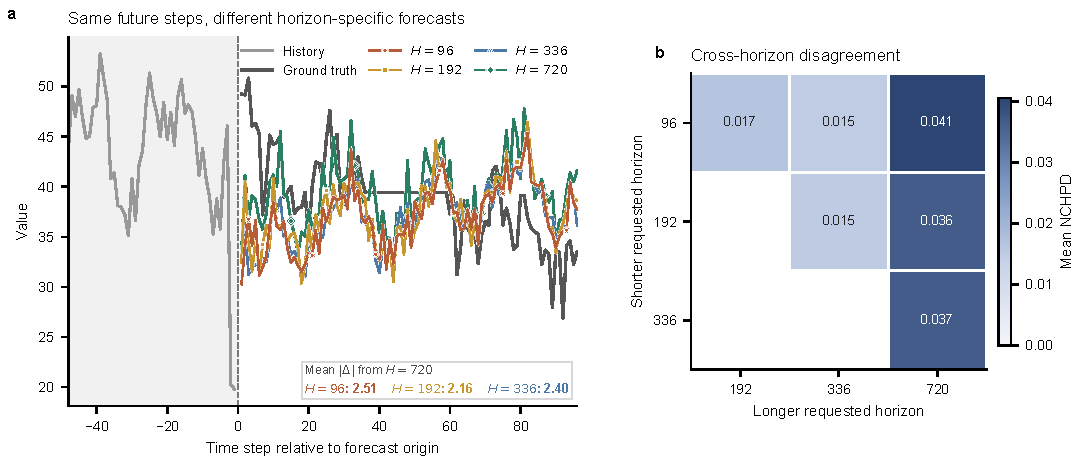
\includegraphics[width=0.96\textwidth]{figures/figure_02_prefix_disagreement.pdf}
\caption{Independently optimized horizon-specific forecasts are inconsistent on shared future steps. \textbf{a}, An ETTh2 validation trajectory selected by aggregate CHPD, showing predictions from DLinear models trained separately for horizons 96, 192, 336 and 720. The panel includes 48 observed steps and the first 96 shared future steps; the inset reports mean absolute differences from the 720-step forecast. \textbf{b}, NCHPD averaged over all ETTh2 validation origins ($n=2{,}161$) and variables.}
\label{fig:prefix-disagreement}
\end{figure*}


\subsection{Future-region sharing-demand heterogeneity}


CHPC specifies how predictions from different horizon requests should relate, but it does not determine how a unified decoder should construct the shared future trajectory. Simply adapting an architecture designed for one fixed horizon leaves this output-side requirement unresolved: a varied-horizon forecaster must learn from requests spanning short to long endpoints while producing one prefix-consistent trajectory. The decoder is therefore central to how predictive information is organized across the future domain, particularly in determining how broadly each history-conditioned state is reused before step-specific prediction.

We use the \textbf{sharing extent} $s$ to denote the number of future steps that reuse one latent state. A \textbf{future region} $\mathcal B_b\subseteq\{1,\ldots,T\}$ is a contiguous subset of the maximum future domain rather than a requested horizon. Broad sharing can capture persistent trajectory structure but may smooth local variations, whereas fine sharing offers greater local flexibility with weaker cross-step regularization. We refer to variation in the preferred extent across regions as \textbf{future-region sharing-demand heterogeneity}.

To isolate this factor, we construct capacity-matched single-extent predictors that differ only in sharing extent; all other architecture, training and evaluation settings remain identical.

For aligned origin $o$, we define the \textbf{future-region prediction risk} of sharing extent $s$ over region $\mathcal B_b$ as the empirical squared-error loss

\[
R_{o,b,s}
=
\frac{1}{|\mathcal B_b|C}
\sum_{\tau\in\mathcal B_b}
\sum_{c=1}^{C}
\left(
\widehat y_{o+\tau,c}^{(s)}
-
y_{o+\tau,c}
\right)^2.
\]


Operationally, $R_{o,b,s}$ is averaged over all future steps and variables in $\mathcal B_b$ for a given origin; it is an empirical region-level risk rather than an expectation over the data distribution. Lower $R_{o,b,s}$ indicates that extent $s$ better matches region $\mathcal B_b$ within the controlled family. A region-dependent preference appears when $s_{o,b}^{\star}=\arg\min_sR_{o,b,s}$ changes with $b$.

We evaluate the five predictors with $s\in\{1,8,32,128,720\}$ across 12 contiguous 60-step future regions on ETTm2. Fig.~\ref{fig:sharing-heterogeneity}a reports the percentage excess prediction risk of each extent above the lowest-risk extent within each region, with outlined squares marking the region-wise winners. The preferred extents vary across the future domain: each of the five extents wins two or three regions, all ten extent pairs exhibit bidirectional crossings beyond the predefined 0.5\% margin, and the mean best-versus-second-best margin reaches 10.266\%. No fixed extent minimizes prediction risk throughout this controlled example, supporting heterogeneous sharing demand across future regions.



\begin{figure*}[t]
\centering
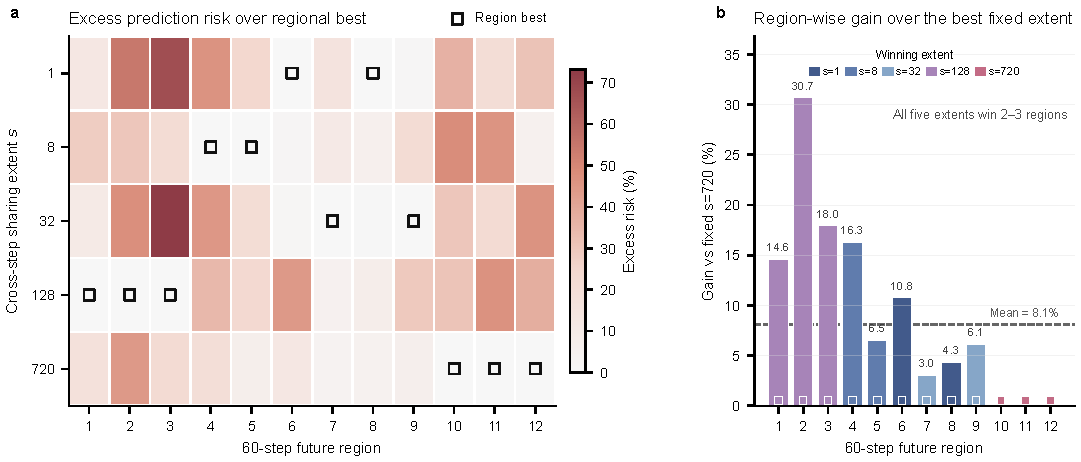
\includegraphics[width=0.96\textwidth]{figures/figure_03_sharing_heterogeneity.pdf}
\caption{Preferred sharing extent varies across future regions. \textbf{a}, Percentage excess future-region prediction risk (mean squared error) of five capacity-matched single-extent predictors above the regional minimum for one selected ETTm2 validation example; outlined squares mark the best extent in each 60-step region. \textbf{b}, MSE reduction obtained by selecting the regional winner instead of the best fixed extent ($s=720$); the dashed line denotes the 12-region mean.}
\label{fig:sharing-heterogeneity}
\end{figure*}


Fig.~\ref{fig:sharing-heterogeneity}b quantifies the performance upper bound associated with these region-wise preferences. Relative to the best fixed extent ($s=720$), selecting the lowest-risk extent separately for each region reduces average MSE by 8.112\%. Because the regional winners are selected using validation labels across separately trained predictors, this value represents descriptive oracle headroom rather than the realized gain of a learned decoder. Within this controlled example, its magnitude nevertheless shows that one fixed extent can leave meaningful region-specific headroom, motivating a decoder that can adapt sharing across the future domain.
